\documentclass{beamer}
\usepackage{lipsum}

\mode<presentation>{\usetheme{Ringerike}}
\usepackage[english]{babel}
\usepackage[latin1]{inputenc}
\usepackage{multicol}
\usepackage{tabularx}

%\usepackage{amsmath,amsthm, amssymb, latexsym}
%\usepackage{lipsum}
%\boldmath
\usepackage[orientation=portrait, size=a0]{beamerposter}

\addtobeamertemplate{block begin}{}{\setlength{\parskip}{30pt plus 1pt minus 1pt}}
\setbeamertemplate{caption}[numbered]

% Bibliography colors and labels
\setbeamertemplate{bibliography item}{\color{white}\ \insertbiblabel}
\setbeamercolor{bibliography entry item}{fg=white}
\setbeamercolor{bibliography entry author}{fg=white}
\setbeamercolor{bibliography entry title}{fg=white} 
\setbeamercolor{bibliography entry location}{fg=white} 
\setbeamercolor{bibliography entry note}{fg=white}

\title{Where}
\subtitle{Software for Geodetic Analysis}
\author{Ingrid Fausk, Michael D\"ahnn, Ann-Silje Kirkvik}
\newcommand{\contact}{ingrid.fausk@kartverket.no\\ {\url https://github.com/kartverket/where}}
\institute{Norwegian Mapping Authority, Geodetic Institute}
\date{October 2019}

\usebackgroundtemplate{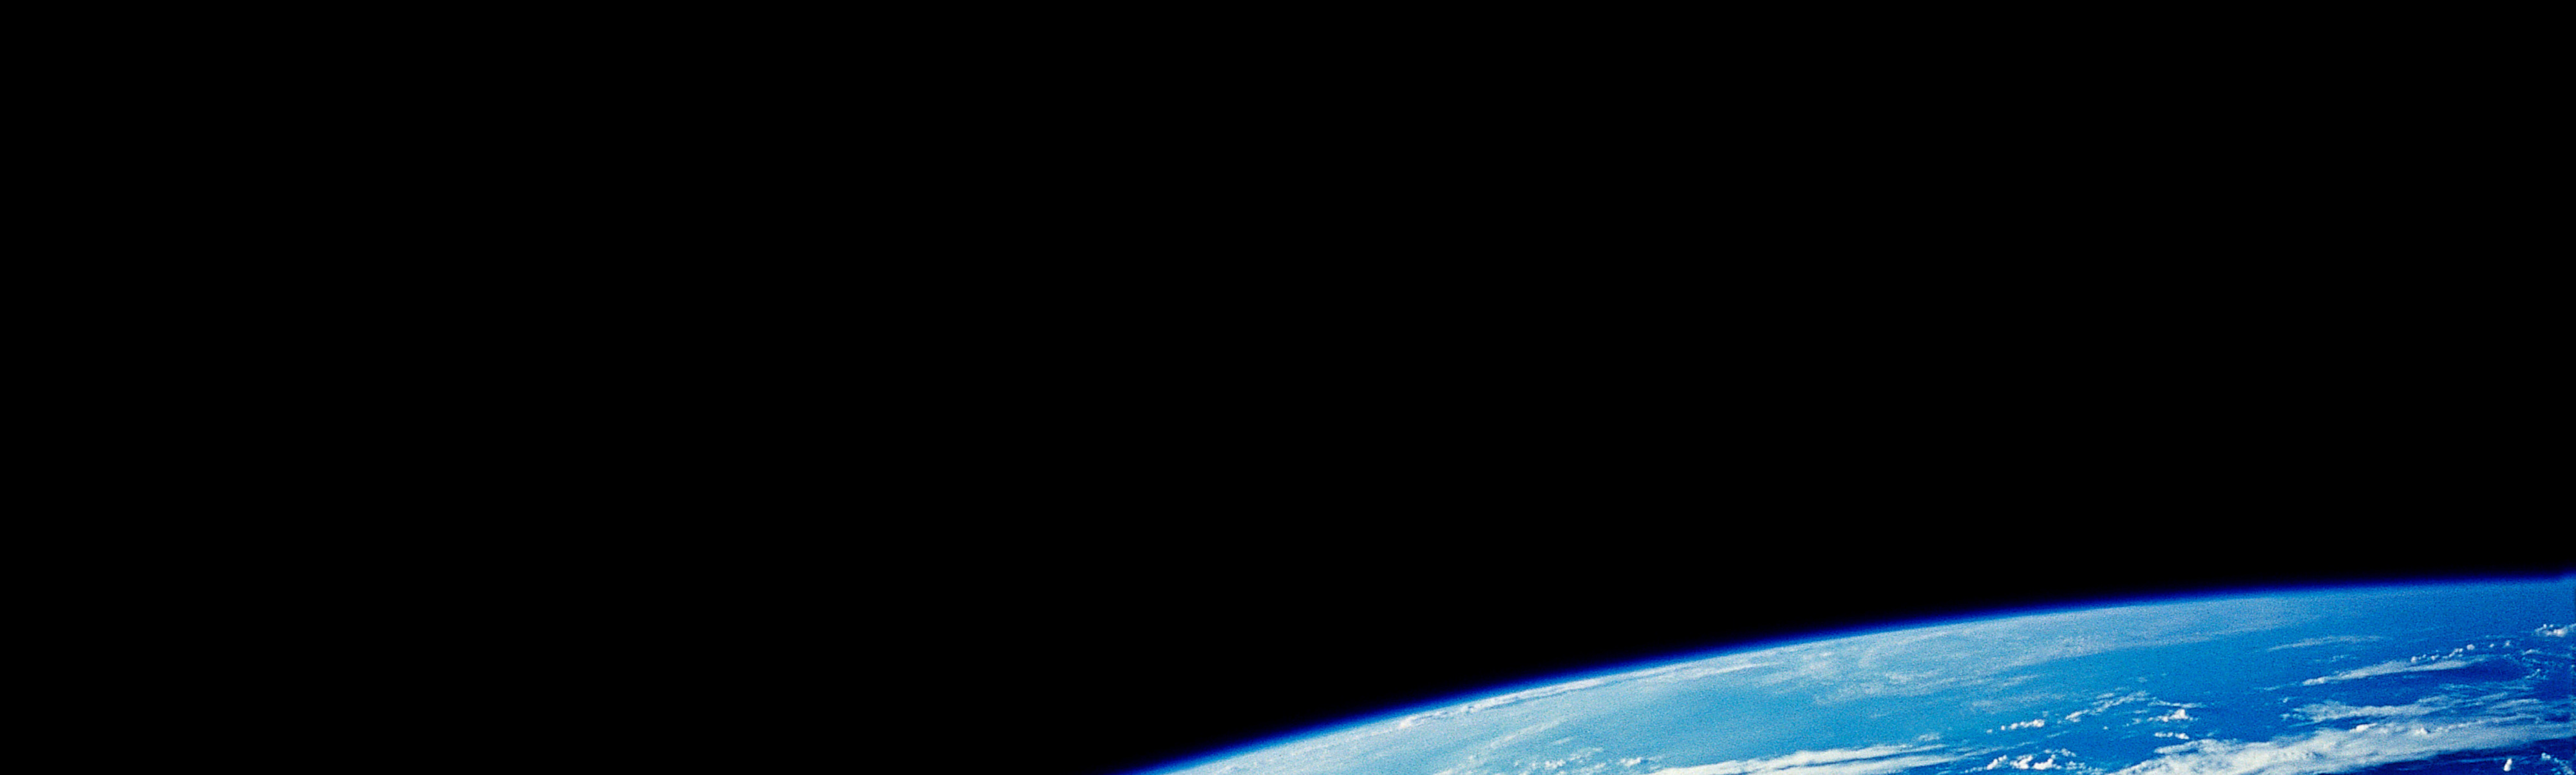
\includegraphics[width=\paperwidth]{figure/earth}}

\begin{document}
\begin{frame}[t]

  % Top title area
  %_____________________________________________________________________________________________
  \color{white}
  \vspace*{4cm}
  \begin{columns}
    \begin{column}[t]{.97\textwidth}
      {\bfseries\fontsize{88}{120}\selectfont \inserttitle}
      {\fontsize{88}{120}\selectfont\kern2cm---\kern2cm\insertsubtitle}
    \end{column}
  \end{columns}

  \vspace*{2cm}
  \begin{columns}
    \begin{column}[t]{.24\textwidth}
      {\fontsize{30}{36}\selectfont\insertauthor\\[0.5cm]
        \fontsize{30}{36}\selectfont{\itshape\insertinstitute}\\ \ \\
        \fontsize{24}{18}\selectfont\texttt{\contact}}\\
        \vspace*{7cm}
        {\color{white}\tiny PHOTO: GETTY IMAGES}
    \end{column}

    \begin{column}[t]{.70\textwidth}
      {\fontsize{30}{36}\selectfont\setlength{\parskip}{15pt}Where is currently being developed at the Norwegian Mapping Authority (Kartverket). The software is written in Python, which has proved very fruitful. The code is quick to write and the architecture is easily extendable
and maintainable, while at the same time taking advantage of well-tested libraries
like the SOFA and IERS packages. Where is an open source project.

\vspace*{-10cm}

\endinput
}
    \end{column}

  \end{columns}
  
  \vspace*{3cm}

  \begin{columns}
    % Content area
    \begin{column}[t]{.9\textwidth}
      \begin{block}{Where}
        \begin{multicols}{2}
          \documentclass[12pt, english]{beamer}

% Packages
\usepackage{xcolor}
\usepackage{eulervm}
\usepackage[utf8]{inputenc}

% Theme
\mode<presentation>
{
  \usetheme{Honefoss}
  \setbeamertemplate{blocks}[rounded]
}

\newcommand{\comment}[1]{{\slshape\color{kvred}#1}}

\title{Where}
\subtitle{A Geodetic Software}
\author{Ingrid Fausk, Michael Dähnn, Ann-Silje Kirkvik}
\date{April 6, 2019}

\begin{document}
\frame[plain]{\titlepage}

\begin{frame}{Where Timeline}
  \begin{itemize}
    \item 2015: Start
    \item 2018: First release as an open source project on GitHub
    \item 2019: Two proposed IVS analysis centers with Where: 
       \begin{itemize}
         \item Kartverket, Norway
         \item Instituto Geográfico Nacional, Spain
       \end{itemize}
    \item 2020: IVS Analysis centers with Where?
    \item 2022: ILRS Analysis center with Where?
  \end{itemize}
\end{frame}

\begin{frame}{Live Demo of Where}
  \begin{itemize}
    \item Running \emph{Where}
    \item Running \emph{There}, a companion tool for visualizing results
    \item Status, discussion
    \item Bugs...
  \end{itemize}
  \begin{figure}
    \begin{flushleft}
      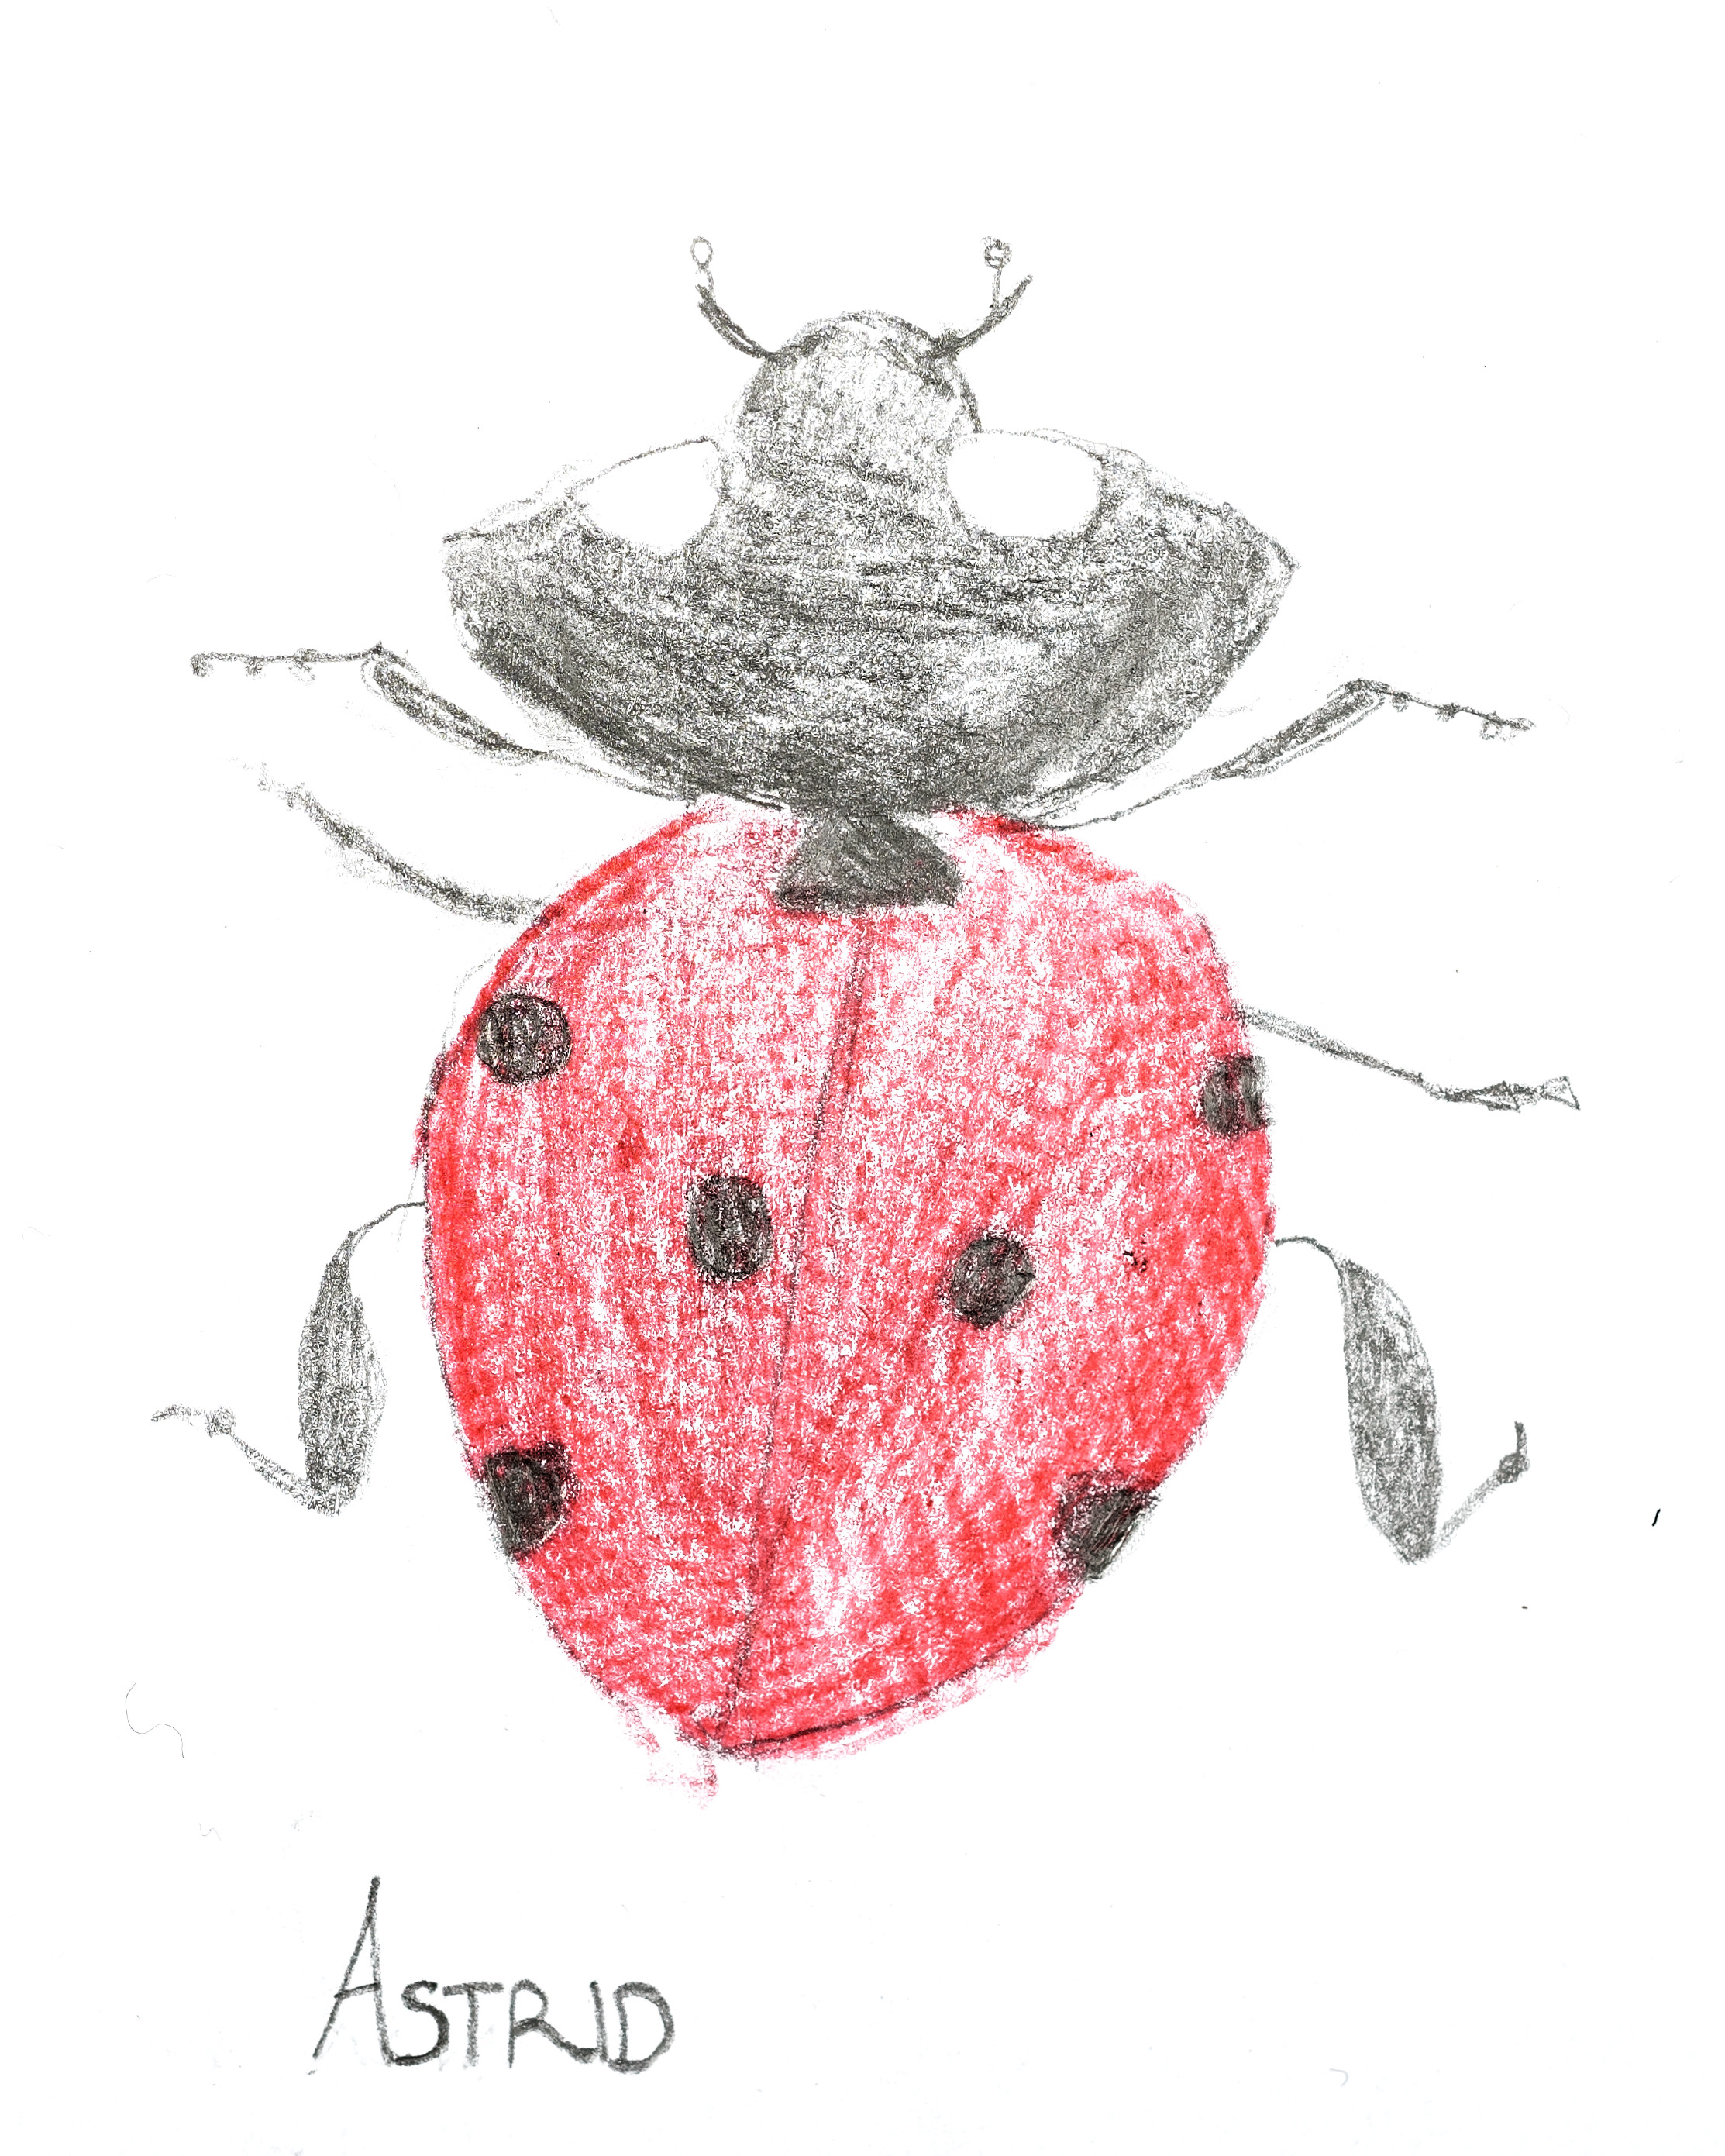
\includegraphics[width=2.5cm]{bug.jpg}
    \end{flushleft}
  \end{figure}     
\end{frame}

\begin{frame}{The Technical Stuff}

The \textbf{Where} software is mainly being written in \emph{Python}

  \begin{itemize}
    \item Cross-platform: Runs on Linux, Mac, Windows
    \item Solid, flexible and fast libraries like \texttt{numpy}, \texttt{astropy}, \texttt{matplotlib} and \texttt{scipy} are available
    \item We use a \textbf{HDF5}-based format for internal data storage
    \item \emph{Python} has effective interfaces to \emph{C} and \emph{Fortran} code, and we use the \textbf{SOFA} and \textbf{IERS} software libraries directly
    \item Orbit integrator using \emph{Cowell} method written in \emph{Python}. 
  \end{itemize}
\end{frame}

\end{document}

        \end{multicols}
      \end{block}
    \end{column}
  \end{columns}
  
  \vspace*{3cm}
 
  \begin{columns}
    \begin{column}[t]{.37\textwidth}

      \begin{figure}
        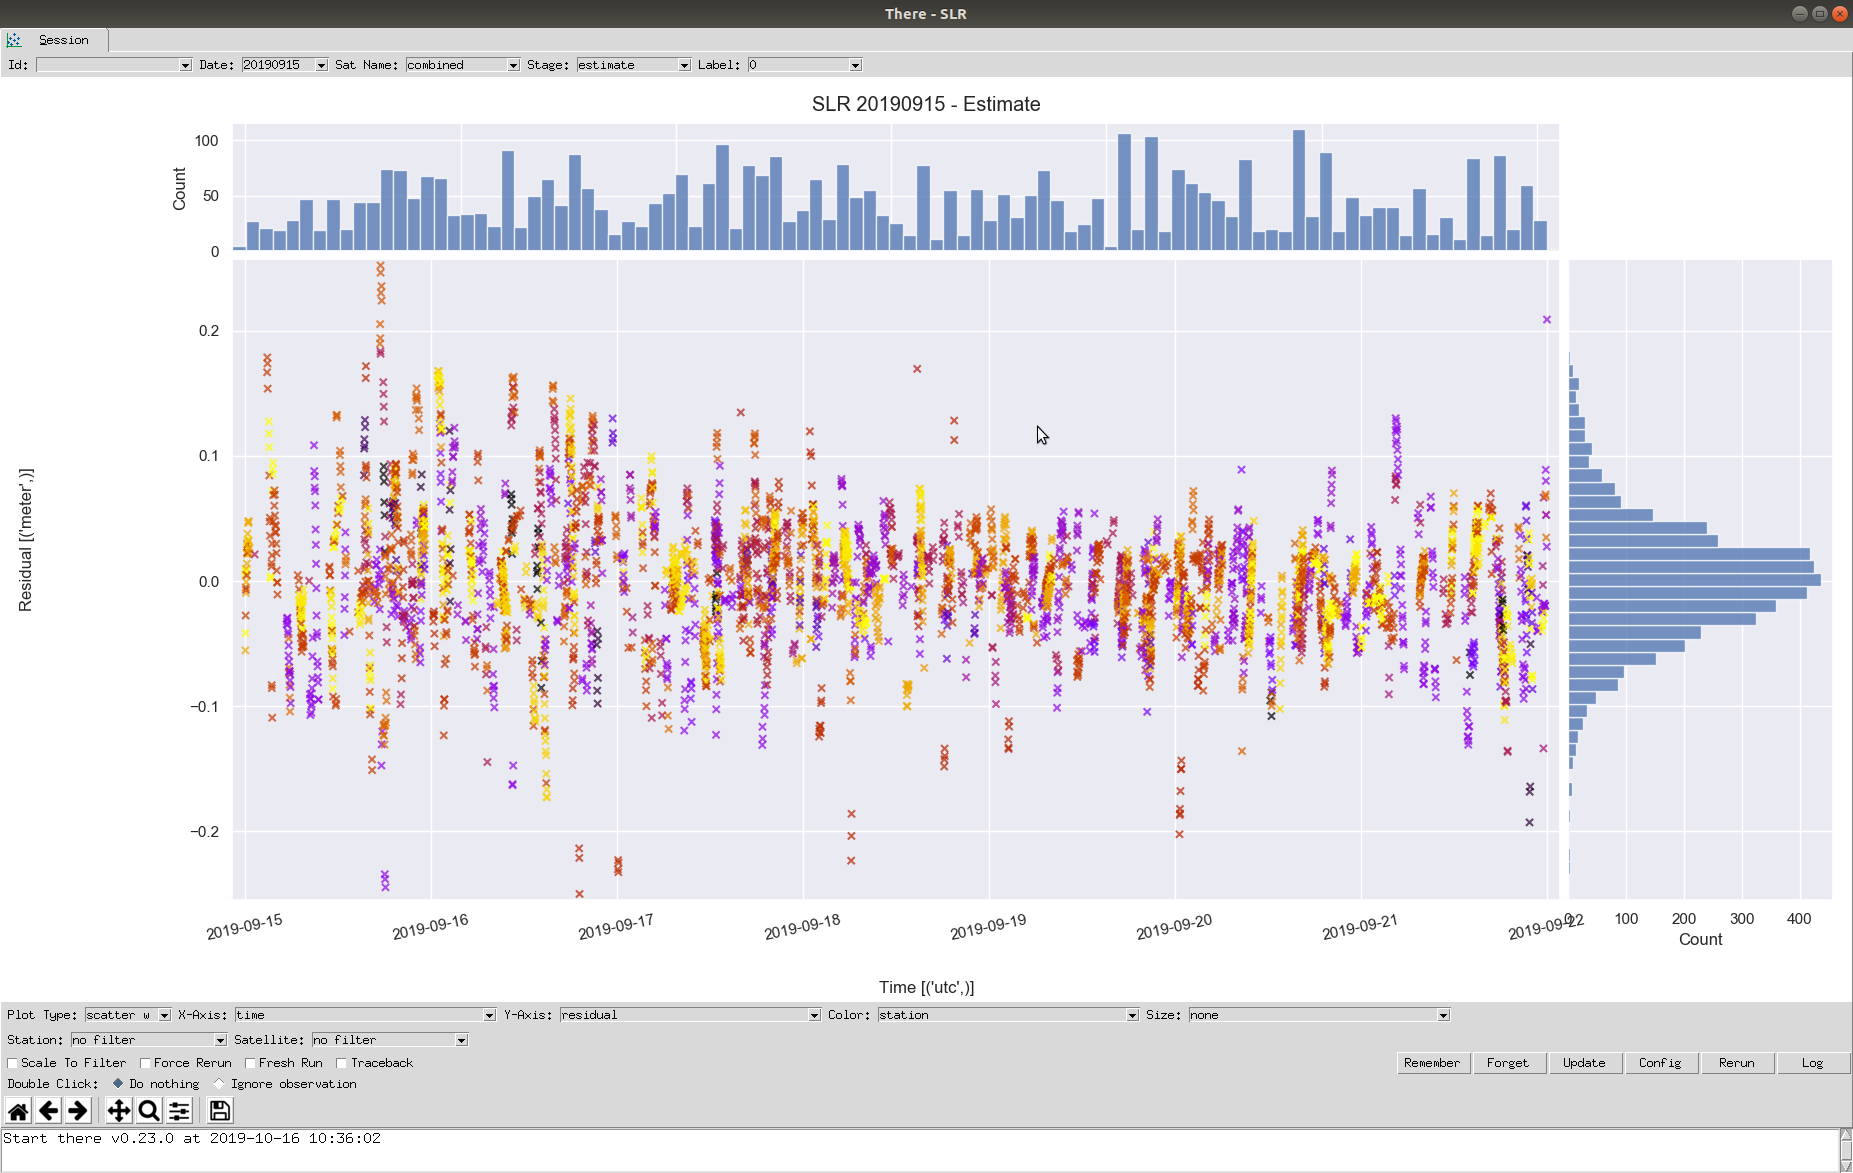
\includegraphics[width=\textwidth]{figure/there}
        \caption{A screenshot of There - a graphical tool developed
	  to look into the results and analysis done by Where. The plot shows
          the observation residuals for the four satellites Lageos1,
          Lageos2, Etalon1 and Etalon2, in meters, for a one week run.} \label{fig:there}
      \end{figure}
    \end{column}
     
    \begin{column}[t]{0.4\textwidth}
      \begin{block}{Future Analysis Centers for VLBI and SLR with Where}
    %    \begin{multicols}{2}
          
The Norwegian Mapping Authority (NMA) is an associated analysis center within
the IVS and ILRS. Both the NMA and the Instituto Geogr\'{a}fico Nacional,
Spain, are in a test phase of deliveries of VLBI analysis results to the IVS
with the Where software. Some of our activities in VLBI is documented
in~\cite{kirkvik2017b} and~\cite{kirkvik2018}. 

Our goal is to be able to contribute to the ILRS after some improvements of the
software, and in the future recieve full status as operational analysis center
for both VLBI and SLR. 

Sharing and cooperating with other institutions is made possible by making
Where an open source project on GitHub.

\endinput

    %    \end{multicols}
      \end{block}
    \end{column}
  \end{columns}

  \vspace*{3cm}
  
  \begin{columns} 
    \begin{column}[t]{.48\textwidth}
      \begin{table}
        \color{black}
\begin{tabularx}{\columnwidth}{l|X}
  EOP & Lagrange interpolation with correction models: Tidal deformation,
  Subdaily tides, Polar motion due to long period ocean tides \\
  \hline
  Orbit models & Earth gravity field (with Solid Earth and Ocean Tides),
  Gravity field of Sun, Moon and planets, Solar radiation, Indirect solar radiation,
  Drag, Relativistic effects, Empirical forces \\
  \hline
  Ephemerides & DE405, DE421, DE430 \\
  \hline
  Displacement models & Atmospheric loading, Eccentricity vector, Ocean loading,
  Ocean pole tides, Solid Earth tides, Solid Earth pole tides \\
  \hline
  Troposphere & GMF, GPT, GPT2, GPT2w, VMF1 \\
  \hline
  VLBI models & Axis offset, Cable calibration, Geometric delay, Gravitational
  delay, Ionosphere, Thermal deformation \\
  \hline
  GNSS models & Antenna correction, Carrier phase wind-up, Ionosphere (higher
  order), Relativistic effects, Range \\
  \hline
  Estimation & Continuous piecewise linear Kalman Filter: Clock, EOP (Polar
  motion, $\Delta$UT1, Nutation), Source direction, Station position, Troposphere
  (Wet delay, Gradients)
\end{tabularx}

\endinput

        \caption{Models and apriori data supported by Where}
        \label{tbl:models}
      \end{table}
    \end{column}

    \begin{column}[t]{.26\textwidth}
      \begin{block}{References}
%        \begin{multicols}{2}
        \footnotesize
\bibliographystyle{../../where}
\bibliography{../../where}
\endinput

%        \end{multicols}
      \end{block}
    \end{column}
  \end{columns}

\end{frame}
\end{document}
